%%%%%%%%%%%%%%%%%%%%%%% file moduleX_template.tex %%%%%%%%%%%%%%%%%
%
%
% This is a template for creating your papers for the course KRW
% It is based on the standard Latex template for Springer publications
% but contains a suggestion for the structure and some content of the
% paper.
%
% Please adapt this document wherever needed.
%
% For more information about the required Latex Style check the document
% typeinst.pdf in the StyleFiles directory.
%
%%%%%%%%%%%%%%%%%%%%%%%%%%%%%%%%%%%%%%%%%%%%%%%%%%%%%%%%%%%%%%%%%%%%%%%%%


\documentclass[runningheads,a4paper]{../../StyleFiles/llncs}

\usepackage{url}
\usepackage{graphicx}
\usepackage{amssymb}	
\usepackage{listings}
\usepackage{multicol}
\lstset{language=SQL,morekeywords={PREFIX,java,rdf,rdfs,url}}


\newcommand{\keywords}[1]{\par\addvspace\baselineskip
\noindent\keywordname\enspace\ignorespaces#1}

\begin{document}

\mainmatter  % start of an individual contribution

% first the title is needed
\title{Data- and Systems Paper: Identifying Handicap Parking Spots for Event's Venues}

% a short form should be given in case it is too long for the running head
\titlerunning{Data- and Systems Paper}

% the name(s) of the author(s) follow(s) next
%
% NB: Chinese authors should write their first names(s) in front of
% their surnames. This ensures that the names appear correctly in
% the running heads and the author index.
%
\author{Alivanistos, Dimitris. \\ Baez, Selene. \\ Jemmett, Andrea. }
%
\authorrunning{Alivanistos, Dimitris. \\ Baez, Selene. \\ Jemmett, Andrea.}
% (feature abused for this document to repeat the title also on left hand pages)

% the affiliations are given next; don't give your e-mail address
% unless you accept that it will be published
\institute{\url{first@vu.nl} \and \url{second@vu.nl}}

\maketitle


\begin{abstract}
The abstract should summarize the contents of the paper and should
contain at least 70 and at most 150 words. It should be written using the
\emph{abstract} environment.
\end{abstract}


\section{Introduction}
% Introduce the sections that follow. What is the core contribution of this paper, and why is that interesting? It is useful to start with a real-life problem, and then explain how your system/dataset (will) solve(s) that problem by means of KR technology. Why is this novel? Has this (or something similar) been done before?
%TODO read WHOLE section again and make it pretty
Amsterdam is a busy city that offers a variety of events and a common problem when attending such events is that Parking Spots are often scarce. Specifically, for handicap people this is an issue that should not be overlooked since they require more time to commute. Hence, having knowledge about close parking spots is specially useful to them. 

However, acquiring this information is not straightforward. The location of venues is not associated with Parking Spot locations, and users usually have to find them themselves by means of maps or driving around. Solving this problem would bring benefits to attendees. %TODO is this novel?

In this project we create a web application that serves as a unique point for finding locations of venues and parking spots related to an event. We decided to work with Museum Galleries and Theaters to keep the scope of the project manageable. To do so we convert existing datasets to RDF format and query them to get the desired results.

In the following section we delve deeper into cases where our proposed solution could be applied. Next, we describe the datasets and continue to explain the data management process to abstract the knowledge from those datasets. Then, we explain the semantics in our data set and provide examples of the queries we used to build the application. We finalize with a demo of the application and a discussion of the work done.  

\section{Scenario / Use Case}
% you could describe the use-case you have in mind that makes use of your chosen data about some matter concerning Amsterdam. Describe the overall idea, but also some concrete usage scenarios (e.g. as part of an actual system). Maybe interaction flow-diagrams etc could be useful, or what is called "personas" https://en.wikipedia.org/wiki/Persona_%28user_experience%29.

As stated in the introduction, the integration of venues and parking spot locations may bring benefits to attendees. Our application will provide a convenient and time-saving option for attendees to find parking spots. Furthermore, by using our application it is guaranteed that the best parking spot will be suggested %TODO not sure about this though ...

Hereby we provide three concrete use-cases where our application's benefits are to be maximized.

\begin{enumerate}
	% Planning in advance
	\item John is in a wheelchair and wants to go to an exhibition in Van Gogh Museum Friday night. John likes to plan things in advance and would like to know where the parking slots closest to the theater are. \\
	The day before the show, John uses our application to find such parking spots and heads to the show confidently. 
	% Quick search once in the theater (on the fly)
	\item Peter broke his leg last month and his friends, as an attempt to cheer him up, invited him to come to a comedy show. He is quite late and is rushing to find the closest parking spots. He quickly browses our application and finds an area with several parking spots. He drives in that direction hoping to find an available spot. 
	% Event manager
	\item Mary is an event organizer who wants to host an exhibition in a Museum next month. She is looking for an accessible venue so she would like to see the distribution of parking spots around the main galleries in Amsterdam. She has a list of five places in mind and uses our application to explore and choose the best venue.
\end{enumerate}


\section{Data sources}
% which datasets have you used and converted? Provide the core properties of those datasets. Also describe other datasets that you might want to integrate, and even data that still needs to be found, or even created.
We decided to integrate the Gemeente's open data about theater events, museums and galleries and handicap's parking slots. Those datasets are available in CSV or JSON formats. We chose to convert from the JSON format because it is a more powerful representation than CSV and because JSON and RDF formats can be easily mapped one to another.

\subsection{Theaters, Museums and Galleries Dataset}
The theaters and museums dataset contains the main features according to the JSON we used:  

\begin{center}
	\textbf{\emph{Features}}
\begin{multicols}{2}
	\begin{enumerate}
		\item \textbf{Trcid}
		\item \textbf{Title}
		\item \textbf{Details *}
		\item \textbf{Types *}
		\item \textbf{Location *}
		\item \textbf{Urls *}
		\item \textbf{Media *}
		\item \textbf{Dates}
		\item \textbf{Lastupdated}
		\item \textbf{Eigenschappen *} 
		\end{enumerate}
\end{multicols}
\end{center} 

The main features (*) in the JSON format that contain sub-features.
\renewcommand{\labelitemi}{$\bullet$}
\renewcommand{\labelitemii}{$\cdot$}
\renewcommand{\labelitemiii}{$\diamond$}
\renewcommand{\labelitemiv}{$\ast$}
\begin{multicols}{2}
	\begin{itemize}
		\item \textit{Details}\itemsep2pt
		\begin{itemize}\itemsep1pt
			\item language
			\item title
			\item calendarsummary
			\item shortdescription
			\item longdescription
		\end{itemize}
		\item \textit{Types}
		\begin{itemize}\itemsep1pt
			\item type
			\item catid
		\end{itemize}
		\item \textit{Location}
		\begin{itemize}
			\item name
			\item city
			\item address
			\item zipcode
			\item latitude
			\item longitude
		\end{itemize}
		\item \textit{Media}
		\begin{itemize}
			\item url
			\item main
		\end{itemize}
		\item \textit{Eigenschappen}
		\begin{itemize}
			\item Catid
			\item Value
			\item CategoryArea
			\item Category
		\end{itemize}
	\end{itemize}
\end{multicols}

\subsection{Handicap's Parking Slots Dataset}
\begin{center}
	\textbf{\emph{Features}}
	\setlength{\columnsep}{4em}
	\begin{multicols}{2}
		\begin{enumerate}
			\item \textbf{Adres}
			\item \textbf{Location}
			\item \textbf{Aantal}
			\item \textbf{Onderbord}
			\item \textbf{Stadsdeel}	
			\item \textbf{Locatie-info}				
		\end{enumerate}
	\end{multicols}
\end{center} 

\section{Building Knowledge Graphs}
% Give details about the data curation and conversion process: which (parts of the) data have you converted, why and how. Which tools did you use? If you wrote your own code, provide a pointer to it. You might wish to add subsections discussing conceptual and technical problems in this process.

\section{Semantic considerations}
% In the 2nd and 3rd lectures we introduced formal Semantics for RDF, RDFS and SPARQL. Please use your own knowledge graph to give some (simple) examples for entailment. Choose a subgraph G (feel free to adapt it if needed) and explain what it stands for, and what the intended meaning is. Given the problem and use-case you have in mind, how do the examples of entailment contribute to a solution?
Here is our vocabulary (Figure \ref{fig:ontology})

\begin{figure}[h]
	\centering
	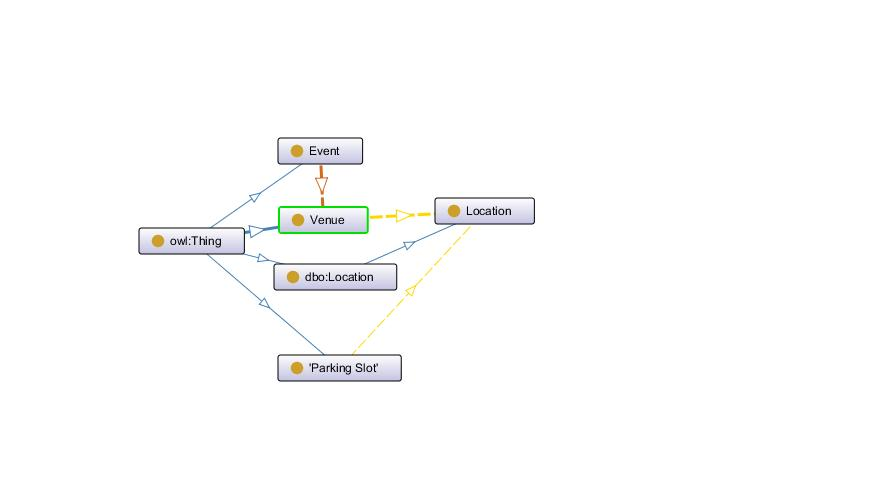
\includegraphics[width=1\textwidth]{img/ontology.jpg}
	\caption{Visualization of the Ontology graph}
	\label{fig:ontology}
\end{figure}

\subsection{RDF and RDFS entailment}
% Give a small graph G' which is entailed by your subgraph G. Feel free to use the same G' that you want to use in your SPARQL query later. Explain why G' is entailed (this is really simple).

% Extend G with a few RDFS triples T={t1,...,tn} and provide a small graph G'' so that G u T |= G'' but not G u T |= G'.

\subsection{SPARQL}
% Give a SPARQL query that provides different answers on the basis of interpreting the knowledge graph with an RDF entailment regime as opposed to an RDFS regime, and explain why you get different answers.

\begin{lstlisting}[captionpos=b, caption=SPARQL query, label=lst:sparql,
basicstyle=\ttfamily,frame=bt]
prefix rdf: <http://www.w3.org/1999/02/22-rdf-syntax-ns#>
prefix owl: <http://www.w3.org/2002/07/owl#>
prefix xsd: <http://www.w3.org/2001/XMLSchema#>
prefix rdfs: <http://www.w3.org/2000/01/rdf-schema#>

prefix : <http://data.krw.d2s.labs.vu.nl/group6/findaslot/vocab/>
prefix data: <http://data.krw.d2s.labs.vu.nl/group6/findaslot/resource/>
prefix geo: <http://www.w3.org/2003/01/geo/wgs84_pos#>
prefix math: <http://www.w3.org/2005/xpath-functions/math#>
prefix dbo: <http://dbpedia.org/ontology/>

select distinct ?venue ?slot ?slat ?slong ?elat ?elong ?dist
where {
?eslot a :ParkingSlot .
?eslot rdfs:label ?slot .
?eslot dbo:location ?slocation .
?slocation geo:lat ?slat ; geo:long ?slong .

data:Podium_Mozaïek a :Venue .
data:Podium_Mozaïek rdfs:label ?venue .
data:Podium_Mozaïek dbo:location ?elocation .
?elocation geo:lat ?elat ; geo:long ?elong .

bind(xsd:double(?slat) * math:pi() / xsd:double(180) as ?la1) .
bind(xsd:double(?slong) * math:pi() / xsd:double(180) as ?lo1) .
bind(xsd:double(?elat) * math:pi() / xsd:double(180) as ?la2) .
bind(xsd:double(?elong) * math:pi() / xsd:double(180) as ?lo2) .
bind(?lo2 - ?lo1 as ?l) .
bind(math:acos(math:sin(?la2)*math:sin(?la1) + math:cos(?la1)*math:cos(?la1)*math:cos(?l)) * xsd:double(6371000) as ?dist) .
}
order by ?dist

\end{lstlisting}


% What is the relation between this fact in terms of model checking and reasoning?

% Investigate and discuss whether there are interesting cases of entailment in your own data.

\section{Discussion}
% Here you summarize the preceding sections, describe the lessons learnt and discuss future work.
% Present a screenshot of a mock-up or working (preferred!) version of your system an describe what it does.
% Argue why the preceding sections show that your solution (partially) solves the problem you introduced in the introduction.

\bibliographystyle{plain}
\bibliography{bibliography}

\end{document}
